\documentclass{article}
\usepackage[english]{babel}
\usepackage[letterpaper,top=2cm,bottom=2cm,left=3cm,right=3cm,marginparwidth=1.75cm]{geometry}
\usepackage{amsmath}
\usepackage{setspace}
\usepackage[colorlinks=true, allcolors=blue]{hyperref}
\usepackage{graphicx}
\usepackage{listings}
\usepackage{subcaption}
\lstdefinestyle{racket-source-code}{basicstyle=\ttfamily\tiny}
\UseRawInputEncoding 

\title{\uppercase{Fitting Regimes into L1 cache}}
\author{Zane Enders & Professor Panchekha}
\date{\today}

\doublespacing
\begin{document}


\begin{titlepage}
    \begin{center}
    

       \vspace*{1cm}

        \textbf{\uppercase{Fitting Regimes into L1 cache}}

       \vspace{0.5cm}
       
       \text{Zane Enders \& Pavel Panchekha}
       
       \date{\today}
            
       \vspace{1.5cm}

   
        A Senior Thesis Submitted to the Faculty of 
        The University of Utah
        In Partial Fulfillment of the Requirements for the
        Degree of Bachelor of Science
        In
        Computer Science
            
       \vspace{0.8cm}
            
       \vfill
    \end{center}
\end{titlepage}
\newpage

\pagenumbering{arabic}

\section{Abstract}
% Sumerize the Study
Herbie\cite{Herbie} is a compiler, developed at the University of Utah and the University of Washington,  leveraging rule-based AI techniques to help with Floating Point accuracy and execution speed for arbitrary math expressions. Floating Point arithmetic is used widely across the industry in fields like numerics to popular large language models. Floating Point covers most of the surface area on hardware. We targeted a bottleneck in the Herbie pipeline in a phase called regimes and reduced its runtime by 3x and its memory usage by 7x.

\section{Introduction}
% TODO Rework this and maybe the intro
When computing the hypotenuse of a triangle using the equation $\sqrt{a^2 + b^2}$ and its Floating Point translation will introduce a surprising amount of error as you can see in figure \ref{fig:hypot-error-graph}. Herbie aims to improve the Floating Point accuracy of arbitrary math expressions using rules-based machine learning techniques leveraging equivalence graphs (eGraphs). To introduce Floating Point error let's start with the hypotenuse of a triangle example. The squiggly line in the middle of figure \ref{fig:hypot-error-graph}.  is the $\%accuracy$ of the expression using 8,000 points sampled by Herbie. As you can see the accuracy of your result is rarely correct on average and as the inputs approach positive and negative infinity, the output is just wrong. Finding the hypotenuse of a triangle is common enough that it has more correct solutions available in math libraries as the function $hypot(a,b)$ which implements a more complex but more correct solution. Not every expression we encounter in this world is lucky or common enough to have a library solution like this example does. This is where Herbie and Odyssey aim to help, both used in exploring alternatives to a given specification like $\sqrt{a^2 + b^2}$, and also help understand where the error in an expression is and insights as to why the error is occurring at that expression.
% TODO site Bhargav's Error Explanations paper?

\begin{figure}[ht]
\centering
\begin{minipage}{0.45\textwidth}
  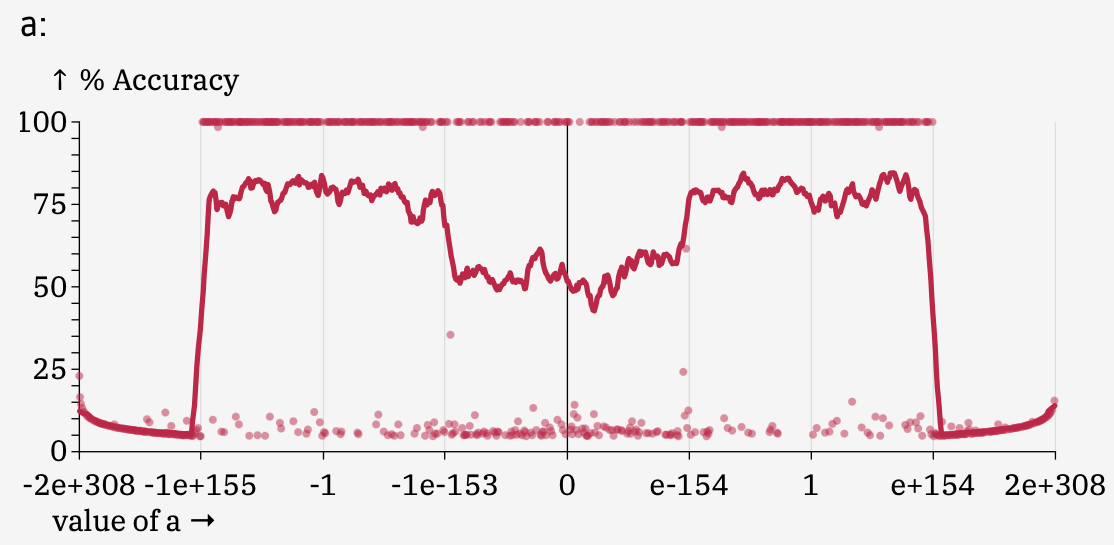
\includegraphics[width=\textwidth]{hypot-error-a.png}
\end{minipage}
\hfill
\begin{minipage}{0.45\textwidth}
  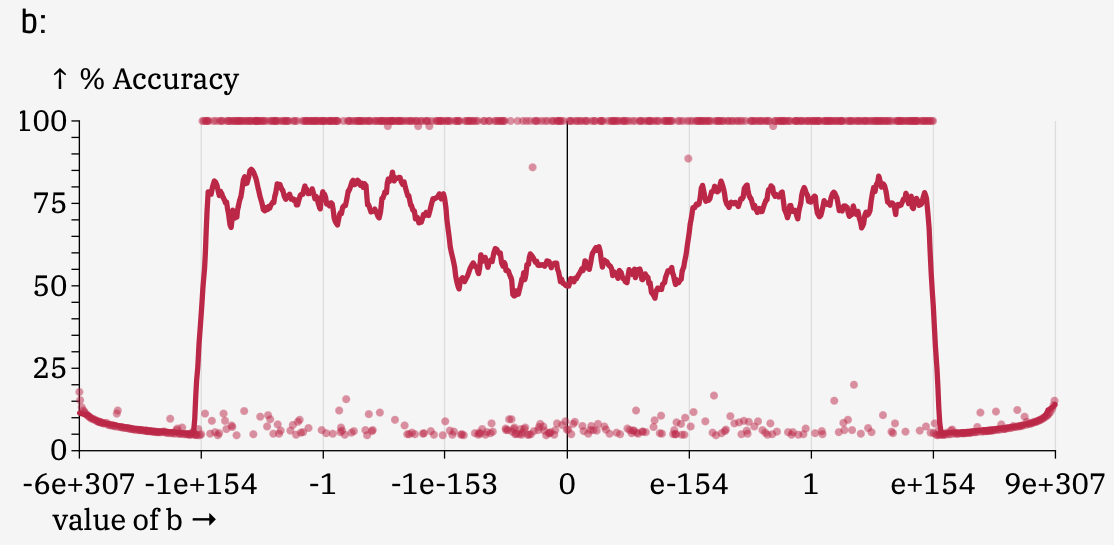
\includegraphics[width=\textwidth]{hypot-error-b.png}
\end{minipage}
\caption{\%Accuracy graph of the output $\sqrt{a^2 + b^2}$ for inputs $a$ and $b$.}
\label{fig:hypot-error-graph}
\end{figure}

\subsection{Herbie overview}

% Clip figure 1 text from the pipeline image.

Herbie takes in Math formulas like $\sqrt{x + 1} - \sqrt{x}$ , an example used in the Herbie paper pulled from Richard Hamming's \cite{Hamming}'s textbook as a specification for an output Floating Point program. This specification has seven sub-expressions, one for each Math operation. Treating variables $x$ and numeric literals $1$  in this specification as expressions. Numeric literals like $1/3$ have an inherent error in them because you can't fit an infinite repeating decimal in a finite amount of space like 64 bits. 

These sub-expressions are used to break down where the error in the specification is occurring. In this example, the error is located in the subtraction operation because of what is called catastrophic cancellation. This is when the left and right-hand sides of the operation are very close to each other, where the majority of the remaining value is lost in rounding error. 

To attempt to solve this problem Herbie first compiles the specification to a naive Floating Point representation which we will refer to in this paper as its program. Our example $\sqrt{x + 1} - \sqrt{x}$ also has seven nodes in the program one for each expression. To get a baseline of this program's correctness in terms of accuracy, 8,256 uniformly distributed points are sampled between positive and negative infinity unless a sub-domain is provided by the user. These sampled points are used to determine the error between the specification and its program. The specification is evaluated using an Interval Arithmetic library called Rival \cite{Rival}, which provides a correctly rounded answer determined by evaluating the expression using as many bits as needed to get a correctly rounded answer in the specified output type. The default output type is a 64-bit Floating Point number also known as Double-precision. Other representations like Posits \cite{Posit} are supported. These sampled points give Herbie a measure of error between the specification and its program on which to improve. 

The First phase of Herbie is the localize phase which determines which sub-expressions contain the highest error; as mentioned before this is the subtraction sub-expression in our example. Alternative programs for the original program are generated by passing these sub-expressions to an eGraph. An eGraph is an efficient data structure used to find all permutations giving a starting state and a provided list of state transitions. In Herbie, this is in the form of mathematical expressions and algebraically equivalent ways of writing that original expression. One of these algebraic rules could be the distributive property $(a +b) * c \equiv (a * c) + ( a * b)$. 

What's considered a good and bad rewrite depends on what metric Herbie is focused on. We will be focused on accuracy. However, you can imagine other metrics like the runtime speed of a program, where introducing branching or a large amount of operations could be a penalty. These alternatives are then ordered and ranked, pruning the worst alternative by whether there is a better alternative for a given point or if its average error is the highest of the set.

The next phase of the Herbie pipeline is to simplify the output expressions using a subset of the rewrite rules, to remove unhelpful rewrites like repeatedly adding one to an expression when adding another constant once is better. The last part of the main loop, visualized in figure \ref{fig:herbie-pipeline} is the series phase. 

The series phase performs a Taylor series expansion on sub-expressions as their expansion could be more accurate than the original expression. This main loop is repeated multiple times (currently 4 iterations) attempt to find a helpful amount of possible alternatives. 

After the main loop is finished Herbie produces a collection of potentially good alternatives to the original program directive from the specification. The best re-write of our example is the expression $\frac{1}{\sqrt{x} + \sqrt{1 + x}}$, which nearly doubles the original accuracy by removing the subtraction operation. These alternatives are passed into the regimes phase of the compiler, potentially producing new alternatives by branching other alternatives together based on their error in different regions of the input domain. From there the alternatives are passed to the finalize phase where the set of alternatives is cleaned and the result is provided to the consumer of Herbie. This completes a very high-level summary of Herbie and allows us to move into the core of the paper which is the speeding up of the regimes section that comes after the main loop.

\begin{figure}[htbp]
\begin{center}
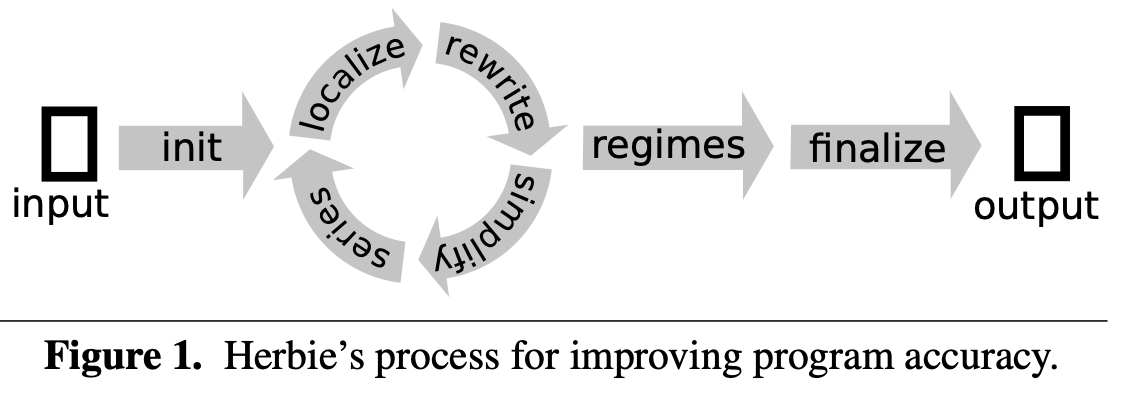
\includegraphics[scale=0.5]{herbie-pipeline.png}
\caption{Herbie's pipeline.}
\label{fig:herbie-pipeline}
\end{center}
\end{figure}

\section{Regimes phase}
The regimes phase is a search over the best alternatives gathered from the main loop visualized in figure \ref{fig:herbie-pipeline}.  Each alternative to the input of regimes is considered to be the most accurate program on at least one of the 256 points pulled from the set of 8,256 original points. The Regimes phase of Herbie is called multiple times with a decreasing subset of the original collection of alternatives. This input set of alternatives are each evaluated based on a summation of their error over 256 possible split points. This provides a cumulative distribution of the error for each alternative, which allows Herbie to use a Least squares approach to minimize the error using a combination of these alternatives to produce an alternative that aims to be more accurate than the original program on average. 

An example of the cumulative error points from seven alternatives evaluated over six possible split points is visualized in figure \ref{fig:cumulative-error}. For each of the six possible split points, we want a line connecting the alternative with the lowest error on each point. When the points of this new line are summed together they aim to have the lowest cumulative error for that set of alternatives.

\begin{figure}[htbp]
\begin{center}
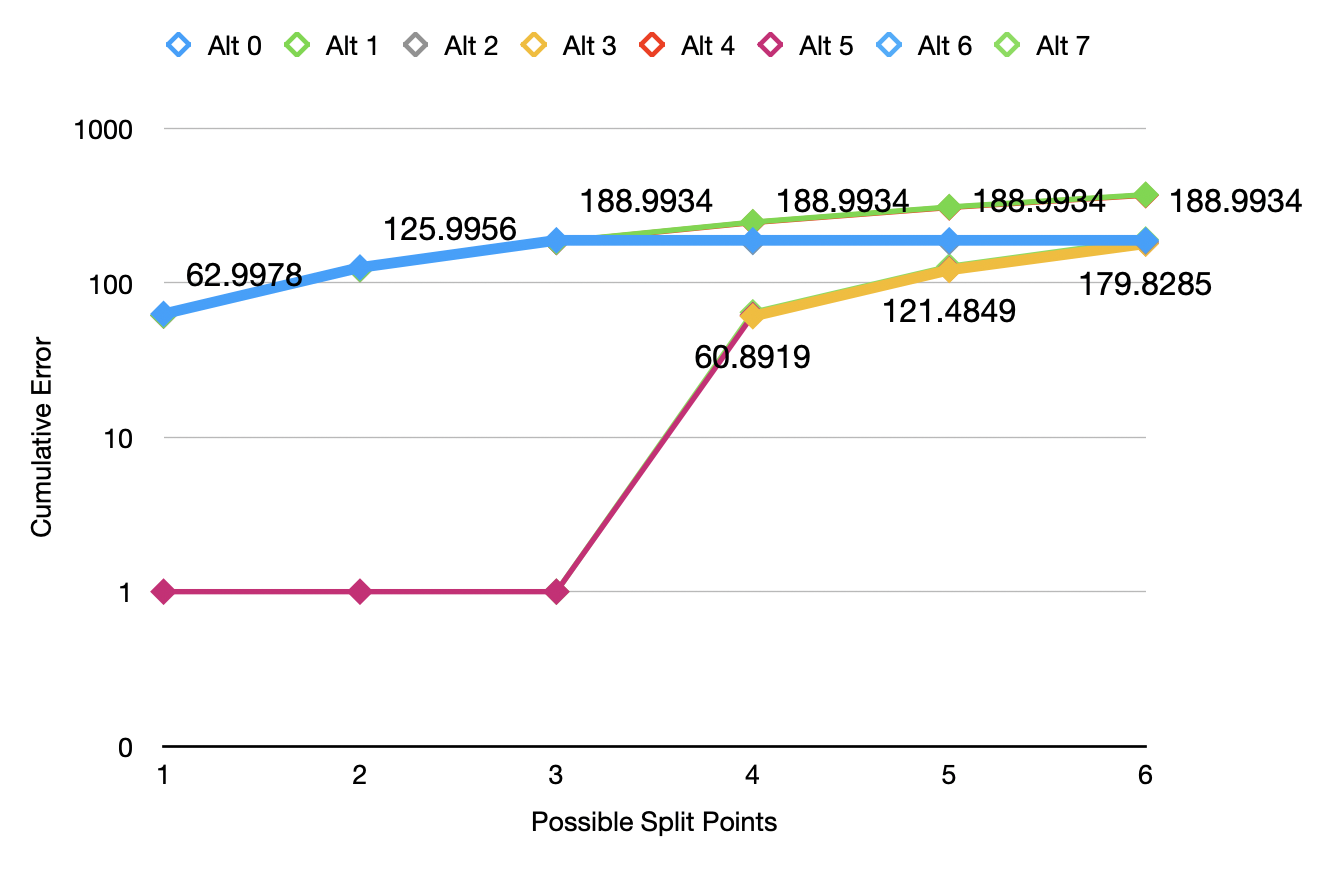
\includegraphics[width=0.95\textwidth]{cumulative-error-graph.png}
\caption{Graph of the cumulative error pulled from Hamming's example with seven alternatives with 6 possible split points. Numbers displaying the two best alternatives. Zeros omitted.}
\label{fig:cumulative-error} 
\end{center}
\end{figure}
% TODO use a different graph that doesn't omit zeros
The greedy algorithm for this is to use the lowest error alternative for each possible split point, but branching between different programs like this has a performance cost so we add a penalty to prevent this behavior. 

This performance cost of branching between programs is due to the CPU changing out the instructions it executes based on the value of a conditional statement. To help with this modern, CPUs can perform what is called speculative execution by running both branches and throwing away the unneeded result, \textit{but this has caused other issues}. The program you are executing is likely to be called more than once so for best performance you want your next instructions to be as close to the CPU as possible, already in the registers ideally or at least in L1 cache.

To give an example of how this can slow things down let's say you are running a function with 1,000,000 inputs and for simplicity's sake we have 250 programs that we are branching between for best accuracy. If these inputs are evenly distributed across the expressions, each expression will be run 4000 times. Depending on the ordering of these inputs they might get executed in nice batches, or you might be unlucky and have to go to L1 between inputs adding roughly 2-3 ns per operation making your computation roughly 2 to 3 times slower than if the inputs were grouped nicely. 

You may not know the distribution of your inputs, but you may know an upper or lower bound on the input in, which case Herbie allows you to add pre-conditions to your specification, which informs Herbie and allows it to better tailor programs for that range. Below is an alternative program produced by regimes from the Hamming example outputted in Python by Herbie. 

\begin{center}
\begin{lstlisting}
if (math.sqrt((x + 1.0)) - math.sqrt(x)) <= 0.05:
  return math.sqrt(math.pow(x, -1.0)) * 0.5
else:
  return math.fma(math.fma(-0.125, x, 0.5), x, (1.0 - math.sqrt(x)))
\end{lstlisting}
\end{center}

\subsection{Original Algorithm}

Source code in Appendix \ref{appendix:old-algorithm}.

The original regime algorithm can be broken into three sections: the initial setup, core loop, and extraction. We have two data types that we are working with, a candidate and split point shown in figure \ref{fig:candidates}. 

The initial setup starts with generating the cumulative error in the form of a fixed-length vector for each alternative. This vector contains the total error of that alternative up to that point. The algorithm loops over each vector representing an alternative selecting the alternative out of the possible alternatives with the lowest cumulative error for that point. We construct what we call a candidate for each of these potential split points. A candidate contains its cumulative error up to that point and a list of split points made before that point to lower the total error. A split point contains the index of which alternative it represents and which point that alternative should be used until. After the initial setup is complete, a list of 256 candidates is generated each containing the cumulative error up to that point and one split point for the alternative that had the lowest cumulative error for that potential split point.

This initial list of candidates is passed to an $add-splitpoint$  function which loops over each of the the possible split points. We loop over the candidate for each point and save its error up to that point as the target to beat for that point. To discourage adding additional split points we subtract a bonus of the total number of possible split points from that candidate's cumulative error. We then loop over all the alternatives for that point and find the alternative with the lowest error for that point, then test if this potential best point beats the cumulative error of the target error to beat.

This inner loop is then repeated until no more changes are made when making successive calls to $add-splitpoint$  when compared to the previous round. This means that no more split points can be added to further lower the error. The last candidate in the output list contains all of the split points of the alternatives needed to obtain the minimum error that it represents. We then return this list of split points to be refined in a binary search phase. This binary search phase refines where the actual split point is to be made. This new alternative returned and added to the other alternatives generated by this call to Herbie.

Below in figure \ref{fig:candidates} shows a final candidate for a reduced test case where 3 alternatives were compared on 5 points. The point indexes in this algorithm base 1 thus why the last point is labeled point 5 instead of 4. On the left is the list of candidates being repeatedly passed into the $add-splitpoint$  function. The resulting candidate with a cumulative error of 551 has its split points in reverse because each candidate starts with one split point representing the best alternative for that point. Splint points are then appended to this list in subsequent calls to $add-splitpoint$  which is where the other split points are added. saying that up to point 1 we should use alternative 1, up to point 2 use alternative 2 and the remaining points use alternative 0.

\begin{figure}[htbp]
\begin{center}
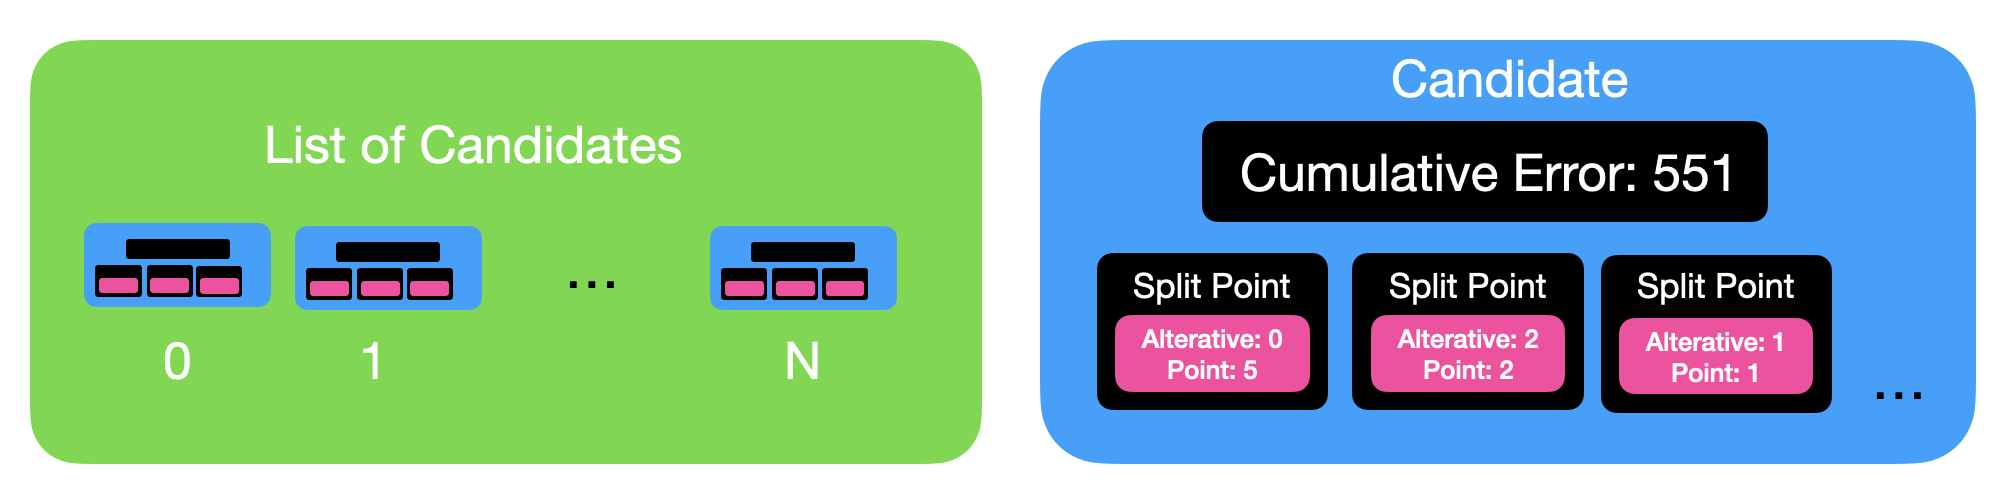
\includegraphics[width=0.95\textwidth]{candidates.png}
\caption{Regimes data structures}
\label{fig:candidates}
\end{center}
\end{figure}

\subsection{Performance gains to be made}
The primary goal of this research is to speed up the regimes section of Herbie. The slowest thing a computer can do in most cases is access information outside of the CPU or its caches. As we aren't doing any networking or disk access for this algorithm the last place to look is if we are allocating to the heap, which we are doing each time we append a new split point to a given candidate inside of three loops that are iterating over the data. 

Allocations to the heap like this can be spread up by pre-allocating the memory before the work in loops is performed. This is the slowdown that we focused on improving when appending a new split point to a candidate's list of split points this can add around 200-300 ns per split point.

To figure out how much memory we could need to allocate ahead of time we can analyze the worst-case scenario of our memory needs. This algorithm works over the two data types, candidates and split points. A split point is two 64-bit integers. A candidate has N main split points and a 64-bit Floating Point value of the cumulative sum of the error for the region it represents. We are working with 256 possible split points so we need space for up to that many split points plus the cumulative error. This requires a total of  $((256 * 2 *8) + 8) * 256 = 1,050,624$ bytes or 1 MB of memory not accounting for some small overhead for language-level booking for garbage collection. A possible final output of  $add-splitpoint$ for a set of three alternatives (0-based index) over five points is visualized in figure \ref{fig:candidate-list}.

\begin{figure}[htbp]
\begin{center}
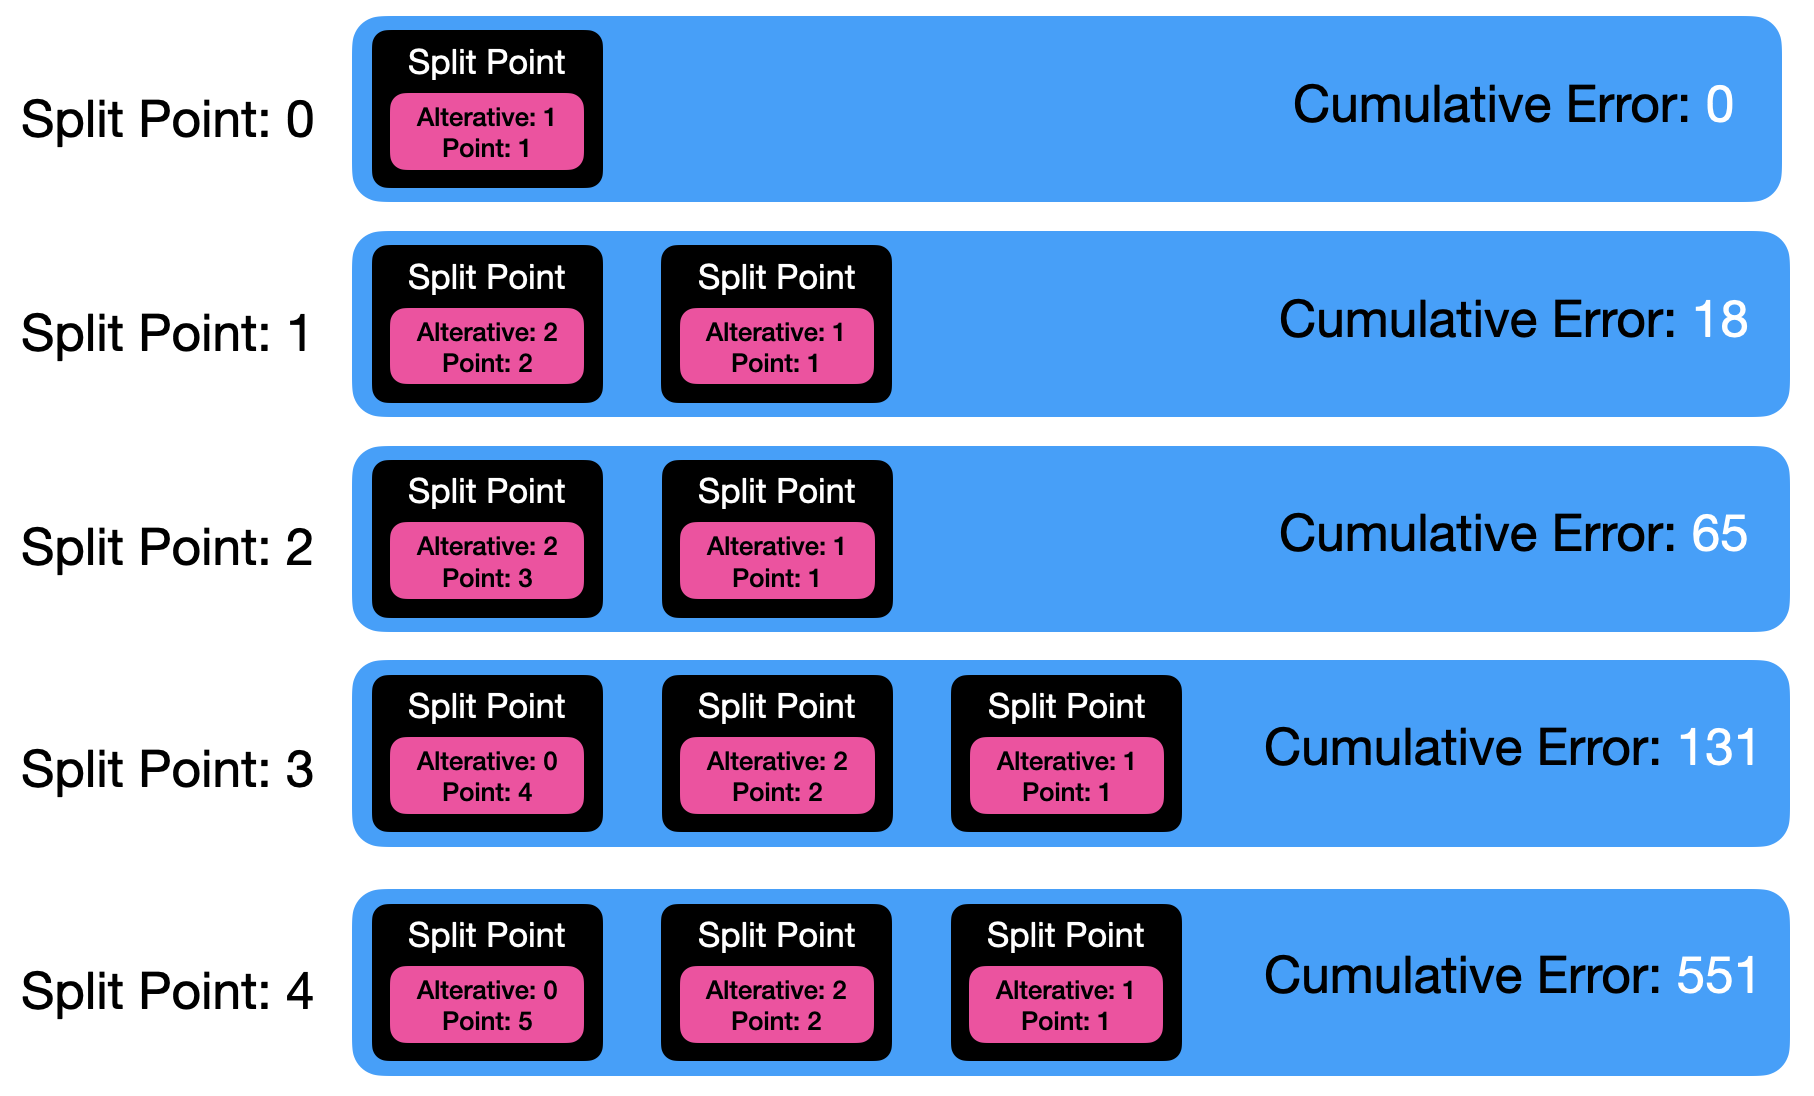
\includegraphics[width=0.8\textwidth]{candidate-list.png}
\caption{State of the candidate list after the algorithm completes starting with 3 alternatives and 5 split points.}
\label{fig:candidate-list} 
\end{center}
\end{figure}

As you can see this data representation contains a bunch of redundant information. For example, we have five occurrences of the split point for an alternative one up to point one. This means we can reduce the amount of memory we need and can potentially fit into the L1 cache, greatly reducing access times and increasing performance. A real output for 256 possible split points will have even more redundant information.

Looking at the fifth candidate labeled split point 4, covering all the possible split points would be the candidate used to generate a new alternative. Its list of split points says that we should use the alternative at index 1 up to point 1, then we should use alternative 2 up to point 2, and finally use alternative zero for the remaining point which is point 5 in this example. 

Looking for what information we need out of figure \ref{fig:candidate-list}, there are 3 categories of information that we are working with: the cumulative error, the candidate index, and the point index. If we flatten this information by their category. We can store this in three vectors, which will have a fixed length of the possible number of split points we are working with and have one vector for each data type. Because these vectors are a fixed size we can allocate them at the beginning of a new algorithm avoiding run time allocations. This new vector-based layout retains the information we need to reconstruct the the output list of split points needed for the next function in Herbie and greatly reduces the data needed to construct this output not to mention much more efficient for the CPU to work with. Dropping from roughly 1 MB down to 768 bytes of information, and thus fitting into the L1 cache. 
Unfortunately, we need a new algorithm to work with our new data layout.

\subsection{New Algorithm}

Source code at Appendix \ref{appendix:new-algorithm}.

The new version of the regimes algorithm doesn’t have as clear distinct phases as the original due to the removal of abstractions to fit into L1. Like the previous version, we still need to generate the cumulative error sum vectors for each alternative. As described before allocate three vectors that initially contain: positive infinity for the cumulative error, zeros for the alternative to use at that point, and the number of possible points in the final vector. Positive infinite for the error at each point which is easy to improve on. Storing zero in the alternative index array as we are guaranteed at least one alternative to start, and we store the max number of points encoding that worst case we use that alternative all points. We then loop over our vectors representing cumulative error representing each possible alternative we could use. Updating our three vectors with the alternative at each point with the lowest error for each point, but still favoring the value that was already there by our penalty value. After this is completed we have a naive set of split points for which we can improve.

For the core of the computation, we create two temporary vectors for which to keep track of the best alternative at a given point, this is used between the next two loops as we loop over all the alternatives. We loop over the three vectors we just set up that are needed to construct our output split point. These two temporary vectors will be reset for each iteration of this loop. One is filled with positive infinite the other with the number of points we are working with (256). These vectors signify the best combination of split points we could find up to the current point of the outer loop. These two temporary vectors will contain the alt with the lowest increase in error and that delete of error for using it at that point. Not adjusted with the penalty yet.

For each point in our output vectors, we loop over all possible alternatives only looking at the alternatives from the start index 0 up to the point index of the outer three vector loop. This defines a sort of sub-range for which we are optimizing. For each point in this sub-range, we compute the delta error of the current alternative for the point we are working on, as our alternatives are represented as a vector of cumulative error we are focusing on just the delta between the previous point and our current point. Looping over all of the candidates we save the index and it's increase in error from the previous point. When complete our temporary vectors contain the lowest delta error and the index of which alternative contains it.

We then loop over the points in that sub-range again this time checking if using the alternative we found and its associated delta increase in error which we saved in our temporary vectors. Checking if using that alt lowers the cumulative error, taking the penalty into account. We break potential ties using the previous alternative already selected by the algorithm. After we have iterated over all of the points we are left with our three vectors which contain the cumulative error at each potential split point, the alternative for which that error is from, and which alternative we should use that point. We then loop back over these vectors and construct the split points that the original algorithm was storing explicitly and return that to the calling function. By changing the data layout and adjusting the algorithm accordingly we have successfully increased the performance and efficiency of this hot spot in regimes well not affecting other parts of Herbie

\subsection{Conclusion}

We flattened out a dynamic algorithm from using recursion to using iteration, reduced the redundant information used, and reduced the number of allocations needed to achieve the same output as the original algorithm. We also changed the data dependency within this triple-for-loop algorithm from looping over the possible number of split points to the number of points again and, then the number of alternatives. To the number of points, the number of alternatives, and then the number of points again. The end goal here was to push the alternatives loop all the way to the outermost loop to try to allow for more alternatives but this proved more difficult and we ran out of time. 
Overall we ended up making a 3.5x improvement in speed and a 7x reduction in memory usage, leading to a roughly 28\% speed up to the nightly benchmark suit, a small step for Herbie and a big step for Regimes.
 
\begin{figure}[htbp]
\begin{center}
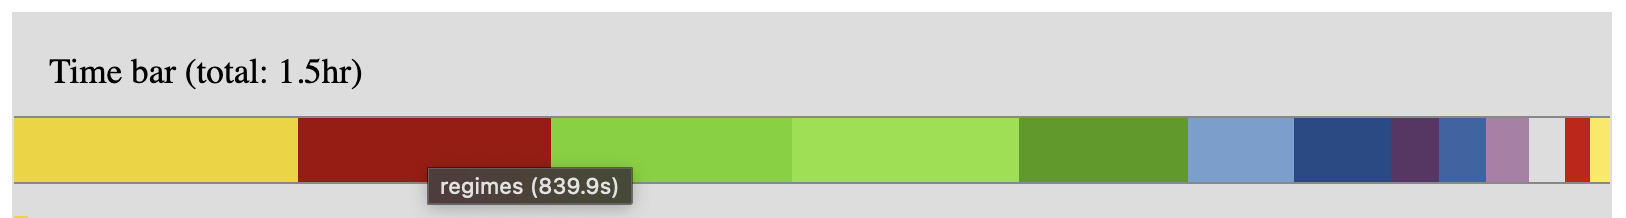
\includegraphics[width=0.95\textwidth]{regimes-before.png}
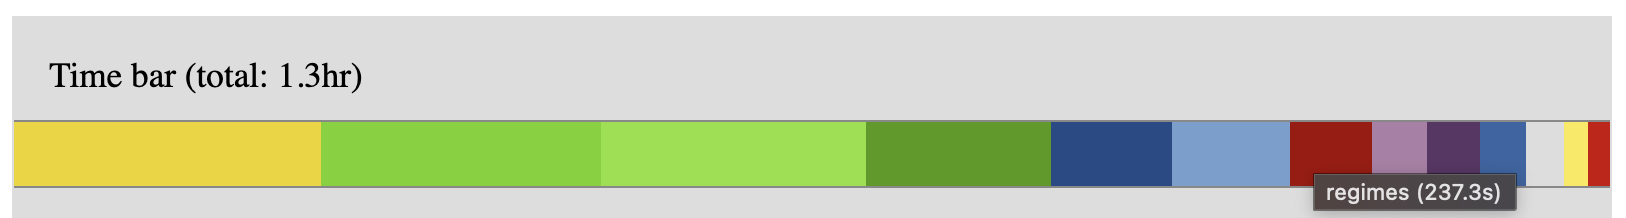
\includegraphics[width=0.95\textwidth]{regimes-after.png}
% TODO put memory usage side by side.

\includegraphics[width=0.80\textwidth]{memory-before.png}

\includegraphics[width=0.80\textwidth]{memory-after.png}
% TODO fix inconsistent memory image size
\caption{Before and after an aggregate of 500+ benchmark expressions.}
% Label is used to reference the image
\label{fig:before-after} 
\end{center}
\end{figure}

\subsection{Future Work}

Future work for regimes could include finish pushing the alternatives loop out to the outermost loop, removing, removing the unnecessary vector of indices to which alternative to use at a given point, and recomputing that at the end. Professor Panchekha made a later attempt at reusing work between calls to regimes that could greatly increase the performance of regimes even further. As this algorithm isn't called just once it is called with a decreasing amount of alternatives, pruning alternatives with a higher average error each call to regimes. So saving work between these calls could save potential work to be computed.

Another avenue of possible future improvements that could be made is tuning the penalty for when to add split points. A nice way of allowing for this would be surfacing this value as an input from a command line flag and later all the way out to a more accessible front end like Odyssey. Allowing the client to experiment with different penalty values and see how that affects the number of branches added and the average error of an expression. Extending this idea; then allows for passing in a vector of weights for each possible split point representing a distribution of their inputs. For example, your program may have to accept inputs ranging from negative infinite to positive infinite but maybe your program has heuristics that say 90\% of the inputs will be between -1 and 1.  This distribution could be passed in as a vector of weights, and the cost of adding a given split point could vary based on this distribution. Having a higher penalty for a split inside the more concentrated area of inputs and a lower penalty for adding branches outside the first quantile.

\bibliographystyle{plain}
\bibliography{citations}
\newpage
\appendix
% TODO Racket source code highlighter?
\lstset{style=racket-source-code}
\section{Regimes Old Algorithm}
Racket source code
\label{appendix:old-algorithm} 
\begin{lstlisting}
(define/contract (err-lsts->split-indices err-lsts can-split-lst)
  (->i ([e (listof list)] [cs (listof boolean?)]) 
        [result (cs) (curry valid-splitindices? cs)])
  (define num-candidates (length err-lsts))
  (define num-points (length (car err-lsts)))
  (define min-weight num-points)
  ; cumulative error sum
  (define psums (map (compose partial-sums list->vector) err-lsts))
  (define can-split? (curry vector-ref (list->vector can-split-lst)))
  
  (define initial
    (for/vector #:length num-points ([point-idx (in-range num-points)])
      (argmin cse-cost
              (map (λ (cand-idx cand-psums)
                     (let ([cost (vector-ref cand-psums point-idx)])
                       (cse cost (list (si cand-idx (+ point-idx 1))))))
                   (range num-candidates)
                   psums))))

  (define (add-splitpoint sp-prev)
    (for/vector #:length num-points
                ([point-idx (in-naturals)]
                 [point-entry (in-vector sp-prev)])
      (let ([acost (- (cse-cost point-entry) min-weight)]
            [aest point-entry])
        (for ([prev-split-idx (in-range 0 point-idx)]
              [prev-entry (in-vector sp-prev)]
              #:when (can-split? (si-pidx (car (cse-indices prev-entry)))))
          (let ([best #f] [bcost #f])
            (for ([cidx (in-naturals)] [psum (in-list psums)])
              (let ([cost (- (vector-ref psum point-idx) 
                             (vector-ref psum prev-split-idx))])
                (when (or (not best) (< cost bcost))
                  (set! bcost cost)
                  (set! best cidx))))
            (when (and (< (+ (cse-cost prev-entry) bcost) acost))
              (set! acost (+ (cse-cost prev-entry) bcost))
              (set! aest (cse acost (cons (si best (+ point-idx 1)) 
                                          (cse-indices prev-entry)))))))
        aest)))
  (define final
    (let loop ([prev initial])
      (let ([next (add-splitpoint prev)])
        (if (equal? prev next)
            next
            (loop next)))))
  (reverse (cse-indices (vector-ref final (- num-points 1)))))
\end{lstlisting}
\newpage
\section{Regimes New Algorithm}
Racket source code
\label{appendix:new-algorithm} 
\begin{lstlisting}
(define/contract (err-lsts->split-indices err-lsts can-split-lst)
  (->i ([e (listof list)] [cs (listof boolean?)]) 
        [result (cs) (curry valid-splitindices? cs)])
  (define can-split-vec (list->vector can-split))
  (define (make-vec-psum lst)
    (flvector-sums (list->flvector lst)))
  ; cumulative error sum
  (define flvec-psums (vector-map make-vec-psum (list->vector err-lsts)))
  (define number-of-points (vector-length can-split-vec))
  (define min-weight (fl number-of-points))
  
  (define result-error-sums (make-flvector number-of-points +inf.0))
  (define result-alt-idxs (make-vector number-of-points 0))
  (define result-prev-idxs (make-vector number-of-points number-of-points))
  
  (for ([alt-idx (in-naturals)]
        [alt-errors (in-vector flvec-psums)])
    (for ([point-idx (in-range number-of-points)]
          [err (in-flvector alt-errors)]
          #:when (< (fl- err min-weight) (flvector-ref result-error-sums point-idx)))
      (flvector-set! result-error-sums point-idx err)
      (vector-set! result-alt-idxs point-idx alt-idx)))

  (define best-alt-idxs (make-vector number-of-points))
  (define best-alt-costs (make-flvector number-of-points))
  (for ([point-idx (in-range 0 number-of-points)]
        [current-alt-error (in-flvector result-error-sums)]
        [current-alt-idx (in-vector result-alt-idxs)]
        [current-prev-idx (in-vector result-prev-idxs)])
    (vector-fill! best-alt-idxs #f)
    (for ([point (in-range number-of-points)])
      (flvector-set! best-alt-costs point +inf.0))
    (for ([alt-idx (in-naturals)]
          [alt-error-sums (in-vector flvec-psums)])
      (for ([prev-split-idx (in-range 0 point-idx)]
            [prev-alt-error-sum (in-flvector alt-error-sums)]
            [best-alt-idx (in-vector best-alt-idxs)]
            [best-alt-cost (in-flvector best-alt-costs)]
            [can-split (in-vector can-split-vec 1)]
            #:when can-split)
        (let ([current-error (fl- (flvector-ref alt-error-sums point-idx) 
                                  prev-alt-error-sum)])
          (when (or (not best-alt-idx) (fl< current-error best-alt-cost))
            (flvector-set! best-alt-costs prev-split-idx current-error)
            (vector-set! best-alt-idxs prev-split-idx alt-idx)))))

    (for ([prev-split-idx (in-range 0 point-idx)]
          [r-error-sum (in-flvector result-error-sums)]
          [best-alt-idx (in-vector best-alt-idxs)]
          [best-alt-cost (in-flvector best-alt-costs)]
          [can-split (in-vector can-split-vec 1)]
          #:when can-split)
      (define set-cond
        (cond
          [(fl< alt-error-sum current-alt-error) #t]
          [(and (fl= alt-error-sum current-alt-error) 
                (> current-alt-idx best-alt-idx)) #t]
          [(and (fl= alt-error-sum current-alt-error)
                (= current-alt-idx best-alt-idx)
                (> current-prev-idx prev-split-idx)) #t]
          [else #f]))
      (when set-cond
        (set! current-alt-error alt-error-sum)
        (set! current-alt-idx best-alt-idx)
        (set! current-prev-idx prev-split-idx)))
    (flvector-set! result-error-sums point-idx current-alt-error)
    (vector-set! result-alt-idxs point-idx current-alt-idx)
    (vector-set! result-prev-idxs point-idx current-prev-idx))

  (define next number-of-points)
  (define split-idexs #f)
  (for ([i (in-range (- number-of-points 1) -1 -1)]
        #:when (= (+ i 1) next))
    (define alt-idx (vector-ref result-alt-idxs i))
    (define split-idx (vector-ref result-prev-idxs i))
    (set! next (+ split-idx 1))
    (set! split-idexs
          (cond
            [(false? split-idexs) (cons (si alt-idx number-of-points) '())]
            [else (cons (si alt-idx (+ i 1)) split-idexs)])))
  split-idexs)
\end{lstlisting}

\end{document}